%%% Lecture Notes for Math 340
%%% Author: Stefan Eng
\documentclass{article}

\usepackage[utf8]{inputenc}
\usepackage[top=1.5in,left=1in,right=1in,bottom=1.5in,headheight=1in]{geometry}
\usepackage{fancyhdr}
\usepackage{amsmath,amsthm,amssymb}
\usepackage{graphicx}
\usepackage{theoremref}
\usepackage{multicol}
\usepackage{enumerate}
\usepackage{hyperref}
\hypersetup{
  pdfborder = {0 0 0},
  colorlinks,
  citecolor=red,
  linkcolor=red,
  urlcolor=red
}

\graphicspath{{./images/}}


% mymacros.sty
\usepackage{math340_macros}

%%%%%%%%%%%%%%%%%%%%%%%%%%%%%

\theoremstyle{plain}
\newtheorem{axiom}{Axiom}
\newtheorem{thm}{Theorem}[section]
\newtheorem{lemma}{Lemma}

\theoremstyle{definition}
\newtheorem{defn}{Definition}[section]
\newtheorem{example}{Example}[section]

\theoremstyle{remark}
\newtheorem*{note}{Note}
\newtheorem*{answer}{Answer}



\renewcommand\qedsymbol{\ensuremath{\blacksquare}}
\setlength\parindent{0pt}

%%% Heading %%%
\pagestyle{fancy}
\rhead{Stefan Eng}

%%%

\begin{document}

% Uncomment when we want title page and table of contents
%% Title page for the Math 340 class notes

\begin{titlepage}
\thispagestyle{empty}
\begin{center}
\textsc{\LARGE \bfseries Introduction to Probability}\\[.3cm]
\HRule \\[.5cm]
\textsc{\large California State University\\Northridge}\\
\HRule \\[1cm]
\textsc{\large Stefan Eng}
\vfill

{\large Fall 2013}

\end{center}
\end{titlepage}

%\tableofcontents
%\vfill
%\pagebreak

\section{Discrete Probability}

%\subsection{Terms}
%Some basic definitions.


%\begin{defn}[Conditional Probability] \thlabel{cond}
%The probability of A occurring given that B already occurred is equivalent to:
%$$
%P(A|B) = \frac{P(A \cap B)}{P(B)}
%$$
%\end{defn}

%\subsection{Set Theory}
%Some basic set theory is needed in the study of probability.

\subsection{Experiment}
The example below of an experiment will describe the various parts of an experiment.
\begin{example}
Assume our \textit{experiment} is rolling one die. Then our \textit{sample space} is as follows:\\
\begin{multicols}{2}
  \begin{tabular}{c|c}
    Simple Events & Prob\\
    \hline\\[-8pt]
    1 & $\frac{1}{6}$\\[2pt]
    2 & $\frac{1}{6}$\\[2pt]
    3 & $\frac{1}{6}$\\[2pt]
    4 & $\frac{1}{6}$\\[2pt]
    5 & $\frac{1}{6}$\\[2pt]
    6 & $\frac{1}{6}$
  \end{tabular}
  \vfill
  \columnbreak
  \underline{Other (non-simple) Events:}\\
  A : dice is even.\\
  $A = \{2,4,6\}$\\
  B : dice is greater than 4.\\
  $B = \{5,6\}$\\
  $P(A) = \frac{1}{6} + \frac{1}{6} + \frac{1}{6}$\\
  $P(B) = \frac{1}{6} + \frac{1}{6}$
\end{multicols}
\end{example}
\subsubsection{Terms}
After seeing an example of what an experiment looks like, now we can see a few definitions.
\begin{defn}[Experiment]
The process by which an observation is made.
\end{defn}

\begin{defn}[Event]
  Something that occurs and is observed in an experiment.
\end{defn}

\begin{defn}[Simple Event]
  An event that cannot be decomposed. One of the possible outcomes from the experiment. 
\end{defn}

\begin{defn}[Sample Space]
The set of all simple events in an experiment. Denoted as $S$.
\end{defn}

\begin{defn}[Mutually Exclusive] \thlabel{excl}
Two events, A and B, are said to be \textbf{mutually exclusive} or \textbf{disjoint} given that:
$$
P(A \cap B) = \emptyset
$$
This means that A and B cannot occur at the same time.
\end{defn}


\subsection{Axioms}
E is an event. $S$ is the sample space. $E \subseteq S$. To every event in $S$ we assign a probability, $P(E)$. Then following axioms hold:
\begin{axiom} \thlabel{axiom1}
The probability of an event is a non-negative real number.
$$
P(E) \in \mathbb{R}, P(E) \geq 0
$$
\end{axiom}

\begin{axiom} \thlabel{axiom2}
Something will always happen.
$$
P(S) = 1
$$
\end{axiom}

\begin{axiom} \thlabel{axiom3}
For countable, disjoint events $E_1,E_2,\ldots$:
$$ 
P(E_1 \cup E_2 \cup \cdots) = \displaystyle \sum_{i=1}^{\infty} P(E_i)
$$
\end{axiom}

\subsection{Sample Point}
The \textit{sample point method} of calculating probability involves calculating all possible ways an event can happen and see what part of the total number of possible events this is.
%\begin{enumerate}

%\end{enumerate}
\subsubsection{Tools for Sample Point}
If we have a sample space that has $N$ points, each with equal probability of occurring, then given a event $E$ contains $n_i$ sample points, the probability of $E$ occurring is:
$$
P(E) = \frac{n_i}{N}
$$
This is the basis for how we will calculate the probability with the following ways to count sample points.

\begin{thm}[$mn$ rule] \thlabel{mn}
With $m$ elements $a_1, a_2, \ldots, a_m$ and $n$ elements $b_1, b_2, \ldots, b_n$, it is possible to form $mn = m \times n$ pairs. This is equivalent to the number of pairs in the Cartesian Product ($A \times B$).
\end{thm}

\begin{figure}[h!]
\centering
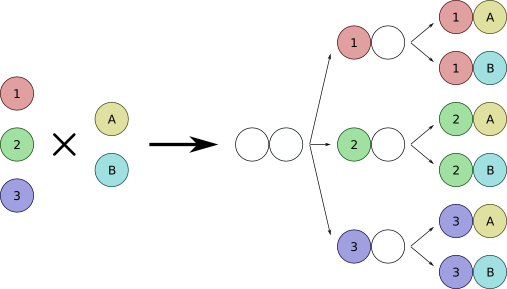
\includegraphics[scale=.5]{counting_mn}
\caption{mn rule}
\label{mn_diagram}
\end{figure}

\begin{defn}[Permutation]
\textit{Ordered} arrangement of k objects from among n object.
$$
\perm{P}{n}{k} = \frac{n!}{n-k!} = n(n-1)\cdots(n-k+1)
$$
\end{defn}
A permutation is very useful when we want to count a sample space where the order matters.
\begin{example}
  Professor Watkins has a class of 30 students. There are 10 front row seats. How many ways are there to seat 10 of the 30 in the front row?
$$
\perm{P}{30}{10} = \frac{30!}{20!} = 30\cdot29\cdot \ldots \cdot 21 \approx 1.09 \times 10^{14}
$$
\end{example}

\begin{defn}[Combination]
\textit{Unordered} subsets of k objects from among k objects.
$$
{n \choose k} = \frac{n!}{k!(n-k)!} = \frac{n (n-1)\cdots (n-k+1)}{k(k-1)\cdots 2}
$$
Which is known as the \textit{binomial coefficient}.
\end{defn}

\begin{example}
In Professor Watkins Math 103 class, 12 students wanted to add the class. He can only add 4 of them. How many different ways can he add the students?
$$
{12 \choose 4} = \frac{12!}{4!\cdot (12-4)!} = 495
$$
So there are 495 different ways he could choose the 4 students to add.
\end{example}

\begin{defn}[Partition]
  If we divide a set of $n$ objects into k distinct subsets containing $n_1,n_2,\ldots,n_k$ objects respectively, such that:
$$
n_1 + n_2 + \ldots + n_k = n
$$
Then the number of ways to partition the set n into k subsets is:
$$
{n \choose {n_1n_2\ldots n_k}} = \frac{n!}{n_1!n_2!\ldots n_k!}
$$
Which is known as the \textit{multinomial coefficient}.
\end{defn}
\begin{example}
In a class of 30 students there will be 4 A's, 6 B's, 18 C's, 2 D's, and 0 F's. How many ways are there to assign these grades?\\
$$n = 30,\ k = 5$$
$$n_1 = 4,\ n_2 = 6,\ n_3 = 18,\ n_4 = 2,\ n_5 = 0$$
$$
{30 \choose {4\ 6\ 18\ 2\ 0}} = \frac{30!}{4!\ 6!\ 18!\ 2!\ 0!} \approx 1.20 \times 10^{12}
$$
In many of these problem there is more than one way to count. We can also count this with combinations and the $mn$ rule (see \thref{mn}).
\begin{center}
${30 \choose 4}$ get A's
${26 \choose 6}$ get B's\\[5pt]
${20 \choose 18}$ get C's
${2 \choose 2}$ get D's

$$
{30 \choose 4}
{26 \choose 6}
{20 \choose 18}
{2 \choose 2} = 1.20 \time 10^{12}
$$
\end{center}
\end{example}

\subsubsection{Method for Sample Point}
The can be used as a reference in how to calculate the probability with the sample point method.
\begin{enumerate}
  \item Define the experiment and determine how to calculate a simple event.
  \item List (or count) the sample space of the simple events, call this $N$.
  \item Assign probabilities to the simple events that satisfy the axioms. Normally the probability is just $\frac{1}{N}$, where $N$ is the number of simple events in the sample space.
  \item Determine what simple events make up the event $A$ we are trying to calculate the probability for. Count or list the number of simple events that make up $A$.
  \item Calculate $P(A)$ with $\frac{|A|}{N}$, or by summing up the probabilities of the sample points.
\end{enumerate}

\subsubsection{Sample Point Examples}
\begin{example}
  A boxcar contains six complex electronic systems. Two of the six are randomly selected for thorough testing and then classified as defective or not defective. 
  \begin{enumerate}[a)]
    \item Two of the six systems are actually defective, find the probability that both are defective.      
    \item What is the probability that at least one of the systems selected is defective?    
  \end{enumerate}
  \begin{answer}[a]
    Given that our sample space has 15 simple events, each with a probability of $\frac{1}{15}$, there is only one way to have two defective components. Therefore, 
    $$
    P(\text{Both defective}) = \frac{1}{15}
    $$
  \end{answer}
  \begin{answer}[b]
    One way to figure out part b is to count the cases where the system does not have any defects and subtract from $|S|$. The number of ways to pick a non-defective system is:
$$
{4 \choose 2} = 6
$$
$$
P(\text{At least one defective}) = \frac{15-6}{15} = \frac{9}{15}
$$
The other way of solving is to list the sample space, and see that there are 9 cases where there is at least one defective component.
  \end{answer}
\end{example}
%\begin{example}
%There are 20 people in a building. What is the probability of one of them having the same birthday as the other? (Assume each day of the year is equally as likely to be born on)
%\begin{answer}
%We are going to approach this problem by counting the probability that the people are born on different days and subtract that from one. First let's start off by counting the number of different ways that the people can be born. Given that there are 365 days in the year (forget about leap year), there are 365 days the first person could be born and 365 the second could be born... we can continue this for all 20 people. So there are $N = (365)^2$ different ways the 20 people could have been born on. 
%\end{answer}
%\end{example}

\subsection{Conditional Probability}
Conditional Probability is best thought of intuitively, built upon the other topics we have looked at.
\begin{example}
  Assume we have a loaded die. The probabilities for this die are as follows:\\
  \begin{center}
    \begin{tabular}{r|c c c c c c}
      & 1 & 2 & 3 & 4 & 5 & 6\\
      \hline
      Prob. & .05 & .20 & .15 & .25 & .05 & .30
    \end{tabular}
  \end{center}
  Let event A : An odd number comes up.
  $$
  P(A) = P(\{1,3,5\}) = .05 + .15 + .05 = .25
  $$
  Let event B : 3 gets rolled.
  $$
  P(B) = P(\{3\}) = .15
  $$
  What is the probability of 3 getting rolled, given that the die is odd? Now the sample space has been restricted. We need some way to \textit{normalize} the next events in the sample space while still following the axioms. One way to think about this process is:
\begin{align*}
P(S) &= 1\\
P(\{1,2,3,4,5,6\}) &= 1\\
P(\{1,3,5\}) + P(\{2,4,6\}) &= 1\\
P(\{1,3,5\}) &= 1 - P(\{2,4,6\})\\
P(\{1,3,5\}) &= 1 - .75\\
P(\{1,3,5\}) &= .25\\
\frac{P(\{1\})}{.25} + \frac{P(\{3\})}{.25} + \frac{P(\{5\})}{.25} &= 1
\end{align*}

Now with our restricted sample space for odd numbers, we have satisfied the axioms by performing a few simple calculations. Now we have a new table of probabilities for our sample space:\\
\begin{center}
    \begin{tabular}{r|c c c}
      & 1 & 3 & 5\\
      \hline\\[-5pt]
      Prob. & $\frac{.05}{.25}$ & $\frac{.15}{.25}$ & $\frac{.05}{.25}$
    \end{tabular}
\end{center}
So clearly now we can see that the probability of B given that A happened is $.60$.
\end{example}

This example was used to show some intuition behind conditional probability. The definition of conditional probability is:
\begin{defn}[Conditional Probability]
For events $A$ and $B$, where $P(B) > 0$, the probability of $A$ given that $B$ occurred is:
$$
P(A|B) = \frac{P(A \cap B)}{P(B)}
$$
\end{defn}

\begin{example}
  Roll two fair dice, one is green and the other is red.\\
  \begin{center}
    \begin{tabular}{r|c c c c c c}
      & 1 & 2 & 3 & 4 & 5 & 6\\  
      \hline
      1 & 1-1 & & $\cdots$ & & & 1-6\\
      2 & 2-1 & & &  & \\
      3 &  & & $\cdots$& & \\
      4 & $\vdots$ & & & & & $\vdots$ \\
      5 & 5-1 & & & & & \\
      6 & 6-1 & & $\cdots$ & & & 6-6
    \end{tabular}
  \end{center}
Each of the simple events have a probability of $\frac{1}{36}$. Some other events are as follows:
\begin{multicols}{2}
  \begin{align*}
    P(\text{Doubles}) &= \frac{6}{36}\\
    P(\text{Sum is 7}) &= \frac{6}{36}\\
    P(\text{Sum is 8}) &= \frac{5}{36}
  \end{align*}
  \vfill
  \columnbreak
  \begin{align*}
    P(\text{Green die is one}) &= \frac{6}{36}\\[7pt]
    P(\text{At least one die is 1} &= \frac{11}{36}
  \end{align*}
\end{multicols}
Which can be verified by the table we have made. Now let's try out some conditional probability(G = Green die, R = Red die):
$$
P(\text{G is 1}|\text{ R is 1}) = \frac{6}{36}
$$
If we look back at the $P(\text{G is 1})$ we see that the result is the same! If the given event has effect on the probability of the first event we say the they are \textbf{independent}.
$$
P(\underbrace{1-1}_{A}|\underbrace{\text{ At least one die is 1}}_{B}) = \frac{1}{11}
$$
If $B$ changes the probability of $A$, then $A$ and $B$ are \textbf{dependent}.
\end{example}

%\begin{example}[Punnett Square]See the \href{http://en.wikipedia.org/wiki/Punnett_square}{Wikipedia Page} if you do not know what a Pennett Square is.
%\begin{center}
%R - Red dominant allele.\\
%r - White recessive allele.\\
%\end{center}
%Given that we have two flowers, both with genotype Rr our Punnett Square will look like this:\\
%\begin{center}
%\begin{tabular}{r|c c}
%& R & r\\
%\hline
%R & RR & Rr\\
%r & Rr & rr
%\end{tabular}
%\end{center}
%\end{example}

\begin{defn}[Conditional Probability] \thlabel{cond}
If we have events A and B, the probability of A given that B occurred is defined as:
$$
P(A|B) = \frac{P(A \cap B)}{P(B)}
$$
\end{defn}

\begin{defn}[Independent] \thlabel{ind}
Two events are \textit{independent} if any one of the following hold:
\begin{align*}
P(A|B) &= P(A)\\
P(B|A) &= P(B)\\
P(A \cap B) &= P(A)P(B)
\end{align*}
Otherwise, the events are said to be \textit{dependent}
\end{defn}

\subsection{Laws}
The following laws are very important for calculating the probability of events.
\begin{thm}[Multiplicative Law of Probability] \thlabel{multi}
The probability of the intersection of two events A and B is
\begin{align*}
P(A \cap B) &= P(A)P(B|A)\\
&= P(B)P(A|B)
\end{align*}
If A and B are \textbf{independent} (see \thref{ind}), then
$$
P(A \cap B) = P(A)P(B)
$$
\end{thm}

\begin{thm}[Additive Law of Probability] \thlabel{add}
The probability of the union of A and B is
$$
P(A \cup B) = P(A) + P(B) - P(A \cap B)
$$
If A and B are \textbf{mutually exclusive} events (see \thref{excl}), $P(A \cap B) = 0$ and
$$
P(A \cup B) = P(A) + P(B)
$$
\end{thm}
\begin{thm}
If A is an event, then
$$
P(A) = 1 - P(\overline{A})
$$
\end{thm}
\begin{proof}
Assume $S$ is a sample space. It follows that $S = A \cup \overline{A}$. Since $A$ and $\overline{A}$ are mutually exclusive events (\thref{excl}), $P(S) = P(A) + P(\overline{A})$. Therefore, $P(A) + P(\overline{A}) = 1$.
\end{proof}

\subsubsection{Event Composition}
Using these laws of probability we can come up with a problem solving strategy.
\begin{enumerate}
\item Define the experiment.
\item Identify some of the sample points if possible.
\item Write the event we are looking for as a composition of two or more events, using intersects, unions and/or complements.
\item Use the Multiplicative(\thref{multi})/Additive(\thref{add}) Law of Probability
\end{enumerate}


\subsection{Bayes' Theorem}
\subsubsection{Intuition}
This example should give us some intuition on how Bayes' Theorem works.
\begin{example}
Suppose a test correctly diagnoses a disease $95\%$ of the time in people who have the disease. Also, if the person does not have the disease, it will report they do not have it $90\%$ of the time. $1\%$ of the population has the disease. If a person is chosen at random and the test indicates that she has the disease, what is the conditional probability that she actually has the disease?

\begin{answer}
First let's start by assigning symbols to the experiment. Let $D$ mean that a person has the disease and $N$ mean the person does not have the disease. Also, let $(+)$ mean the test appeared positive, and $(-)$ mean that the test appeared negative. Then,
\begin{multicols}{3}
\begin{align*}
  P(+|D) &= .95\\
  P(-|D) &= .05
\end{align*}
\vfill
\columnbreak
\begin{align*}
P(-|N) &= .90\\
P(+|N) &= .10
\end{align*}
\vfill
\columnbreak
\begin{align*}
  P(D) &= .01\\
  P(N) &= .99\\
\end{align*}
\vfill
\end{multicols}
We want to know $P(D|+)$. We want to draw a picture such as the one below. (Fill this in with our own information!)
\end{answer}
\end{example}
% Uncomment for tree picture
\begin{figure}[h!]
\centering
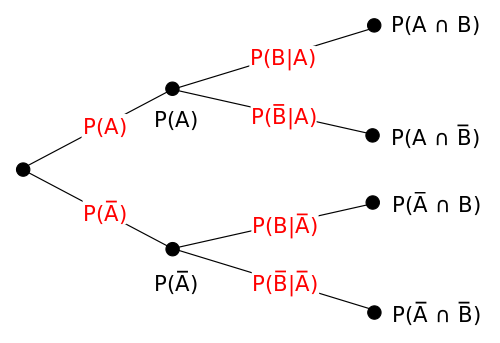
\includegraphics[scale=.5]{tree_diagram}
\caption{Tree Diagram}
\label{tree}
\end{figure}

Finish off this example...

\subsubsection{Formula's and Proofs}
\begin{defn}[Partition] \thlabel{part}
For some positive integer $k$, let the sets $B_1,B_2,\ldots,B_k$ be such that:
\begin{enumerate}
\item $S = B_1 \cup B_2 \cup \cdots B_k$.
\item $B_i \cap B_j = \emptyset$, for $i \not = j$.
\end{enumerate}
\end{defn}

\begin{thm}[Law of Total Probability] \thlabel{totalprob}
  Assume that $\{B_1, B_2, \ldots, B_k\}$ is a partition of S (see Definition \thref{part}) such that $P(B_i) > 0$, for $i = 1, 2, \ldots,k$. Then for any event $A$.
  $$
  P(A) = \displaystyle \sum_{i=1}^k P(A|B_i) P(B_i)
  $$
  or, alternatively,
  $$
  P(A) = \displaystyle \sum_{i=1}^k P(A \cap B_i)
  $$
\end{thm}
\begin{proof}
  Assume A is a subset of S. Then we can write A as:
  \begin{align*}
    A &= A \cap S\\
      &= A \cap (B_1 \cup B_2 \cup \cdots \cup B_k)\\
      &= (A \cap B_1) \cup (A \cap B_2) \cup \cdots \cup (A \cap B_k)
  \end{align*}
  Since $\{B_1, B_2, \ldots, B_k\}$ is a partition of S, if $i \not = j$,
  \begin{align*}
    (A \cap B_i) \cap (A \cap B_j) &= A \cap (B_i \cap B_j)\\
    &= A \cap \emptyset\\
    &= \emptyset
  \end{align*}
  Thus, $(A \cap B_1)$ and $(A \cap B_j)$ are mutually exclusive events (see \thref{excl}). It follows that,
  \begin{align*}
    P(A) &= P(A \cap B_1) + P(A \cap B_2) + \cdots + P(A \cap B_k)\\
    &= P(A|B_1)P(B_1) + P(A|B_2)P(B_2) + \cdots + P(A|B_k)P(B_k)\\
    &= \displaystyle \sum_{i=1}^k P(A|B_i)P(B_i)
  \end{align*}
\end{proof}

\begin{note}
The Law of Total Probability is used when $P(A|B_i)$ is easier to calculate then $P(A)$.
\end{note}

\begin{thm}[Bayes' Theorem] \thlabel{bayes}
Assume that $\{B_1,B_2,\ldots,B_k\}$ is a \textbf{partition} of S (see \thref{part}) such that $P(B_i) > 0$, for $i = 1,2,\ldots,k$. Then
$$
P(B_i|A) = \frac{P(A|B_j)P(B_j)}{\displaystyle \sum_{i = 1}^k P(A|B_i)P(B_i)}
$$
\end{thm}
\begin{proof}
The proof follows from the definition of conditional probability (see \thref{cond}) and the law of total probability (see \thref{totalprob}).
\begin{align*}
P(B_j|A) &= \frac{P(A \cap B_j)}{P(A)}\\[5pt]
&= \frac{P(A|B_j)P(B_j)}{\displaystyle \sum_{i = 1}^k P(A|B_i)P(B_i)}
\end{align*}
\end{proof}

\section{Discrete Random Variables}
\begin{defn}[Discrete Random Variable]
A random variable $Y$ is said to be \textit{discrete} if it can assume only a finite or countably infinite number of distinct values.
\end{defn}

\begin{note}
Random variable will be denoted as such, $(Y = y)$ is the set of all points in $S$ assigned the value $y$ by the random variable $Y$.
\end{note}

\begin{defn}
The \textit{probability} that $Y$ takes on the value $y$, $P(Y = y)$, is defined as the sum of the probabilities of all sample points in $S$ that are assigned the value y. This can also be denoted as, $p(y)$.
\end{defn}

\begin{defn}
The \textit{probability distribution} for a discrete random variable $Y$ can be represented by a formula, table, or a graph that provides $p(y) = P(Y = y)$ for all $y$.
\end{defn}

\begin{thm}
For any discrete probability distribution, the following must be true:
\begin{enumerate}
\item $0 \leq p(y) \leq 1$ for all $y$.
\item $\sum_{y}p(y) = 1$, where the summation is over all values of $y$ with nonzero probability.
\end{enumerate}
\end{thm}

\subsection{Expected Value of a Random Variable}
\begin{defn}[Expected Value] \thlabel{ev}
Let $Y$ be a discrete random variable with the probability function $p(y)$. Then the \textit{expected value} of $Y$, $E(Y)$ is defined as:
$$
E(Y) = \displaystyle \sum_{y}y\cdot p(y)
$$
\end{defn}

\begin{note}
If $p(y)$ is an accurate characterization of the population frequency distribution, then $E(Y) = \mu$.
\end{note}

\begin{defn}
If $Y$ is a random variable with mean $E(Y) = \mu$, the \textbf{variance} of a random variable $Y$ is defined to be the expected value of $(Y - \mu)^2$. That is,
$$
V(Y) = E[(Y - \mu)^2] = \sigma^2
$$
The \textbf{standard deviation} of $Y$ is the positive square root of $V(Y)$, notated as $$
\sigma = \sqrt{V(Y)}
$$.
\end{defn}

\begin{thm}
Given that $c$ is a constant:
$$E[c] = c$$
\end{thm}
\begin{proof}
  \begin{align*}
    E[c] &= \displaystyle \sum_{y} c \cdot p(y)\\
    &= c \displaystyle \sum_{y} p(y)\\   
  \end{align*}
We know that $\sum_{y} p(y) = 1$, therefore $E[c] = c$.
\end{proof}

\begin{thm}
  Let $Y$ be a discrete random variable with probability function $p(y)$ and mean $E(Y) = \mu$. Then:
$$
V(Y) = \sigma^2 = E[(Y - \mu)^2] = E[Y^2] - \mu^2
$$
\end{thm}
\begin{proof}
  \begin{align*}
    \sigma^2 &= E[(Y - \mu)^2]\\
    &= E[Y^2 - 2\mu Y - \mu^2]\\
    &= E[Y^2] - 2\mu E[Y] - \mu^2\\
    &= E[Y^2] - 2 \mu ^2 - \mu^2\\
    &= E[Y^2] - \mu ^2
  \end{align*}
\end{proof}

\subsection{Binomial Experiment}
\begin{defn}[Binomial Experiment] \thlabel{bin_exp} If we have an experiment that satisfies these conditions:
  \begin{enumerate}
    \item The experiment consists of a fixed number, n, of identical trials.
    \item Each trial results in one of two outcomes: \textbf{S} for success and \textbf{F} for failure.
    \item The probability of success is given by $P(S) = p$ and the probability of failure is given as $P(F) = q$, where $q = 1 - p$.
    \item The trials are independent.
    \item The random variable of interested is $Y$, the number of successes observed during $n$ trials.
  \end{enumerate}
  we say that an experiment is a \textbf{binomial experiment}.
\end{defn}

\begin{example}
Insert intuition behind binomial experiment... see notes and page 102-103 of the book.
\end{example}

\begin{defn}[Binomial Distribution] \thlabel{bin_dist}
A random variable $Y$ is said to have a \textbf{binomial distribution} based on $n$ trials with success probability $p$ if and only if:
\begin{align*}
p(y) = {n \choose y} p^y q^{n-y} && y = 0,1,2,\ldots ,n\text{ and }0 \leq p \leq 1.
\end{align*}
\end{defn}

\begin{thm}[Expected Value and Variance] \thlabel{ev_var_bin}
  Let $Y$ be a binomial random variable based on $n$ trials and success probability $p$. Then
$$
\mu = E(Y) = np \text{ and } \sigma^2 = V(Y) = npq
$$
\end{thm}
\begin{proof}
...
\end{proof}

\subsection{Geometric Distribution}
Similar to a binomial experiment the geometric experiment can result in one of two outcomes: success or failure. Probability of success is usually defined as $p$ and failure defined as $q$.
\begin{defn}[Geometric Distribution]
The geometric random variable $Y$ is the number of the trial on which the first success occurs. The experiment consists of a series of trials that concludes with the first success.
\end{defn}
(Insert some stuff about the sample space and intuition behind the formula)
\begin{defn}
  A random variable $Y$ is said to have a \textit{geometric probability distribution} if and only if
\begin{align*}
  p(y) = q^{y-1}p, && y = 1,2,3,\ldots , &&& 0 \leq p < 1.
\end{align*}
\end{defn}

\subsection{Hypergeometric Probability Distribution}

\begin{example}
You draw five cards from a 52-card deck. What is the probability that you get exactly 4 hearts?
\end{example}
\begin{answer}
  Sample space has $52 \choose 5$ simple events. How many of these contain 4 hearts and 1 non-heart:
$$
\frac{ \displaystyle {13 \choose 4} {39 \choose 1} }%
{ \displaystyle {52 \choose 5} }
$$
\end{answer}

%\begin{example}
%  An urn has a total of $N$ balls. $r$ are red and $N-r$ are white. Draw $n$ balls. What's the probability of getting exactly $y$ red balls?
%\end{example}

\begin{defn}[Hypergeometric Probability Distribution]
A random variable $Y$ is said to have a \textit{hypergeometric probability distribution} if and only if:
$$
p(y) = \frac{ \displaystyle {r \choose y} {N - r \choose n - y}} {\displaystyle {N \choose n}}
$$
Where $y$ is an integer $0,1,2,\ldots , n$ subject to the restrictions $y \leq r$ and $n - y \leq N - r$.
\end{defn}

\subsubsection{Memoryless property}

\section{Poisson Distribution}
Suppose we are trying figure out how many cars will pass by a location in some time interval. Let's say we know the average from watching over a long period of time and we determine that it is $\lambda$, which is our expected value. We know from a binomial random variable based on $n$ trials and success probability $p$ that $E(Y) = n \cdot p$ and thus, $E(Y) = \lambda = n \cdot p$. In this case, $n$ is the number of intervals, and $p$ is the probability of a car passing. Since we have a binomial probability:
$$
P(Y = y) = \displaystyle {n \choose y} p^y (1 - p)^{n-y}
$$
It follows from $\lambda = n \dot p$ that:
$$
{n \choose y}%
%
\left( 
  \frac{\lambda}{n} 
\right)^{y}%
%
\left(
  1 - \frac{\lambda}{n}
\right)^{n-y}
$$

Now we are left with the problem of choosing $n$. We only have probability of \textit{one} event happening in $\frac{\lambda}{n}$ time. So if our value for $n$ is too small, then multiple cars could pass by in one time interval. The solution to this is to see what happens when we shorten the time interval to only allow for one car to pass at a time. To decrease $\frac{\lambda}{n}$ to as small as possible, we take the limit as $n$ goes to infinity. (First we need a lemma)
\begin{lemma}
$$\lim_{x \to \infty} \left( 1 + \frac{a}{x} \right)^{x} = e^a$$
Let $\displaystyle \frac{1}{n} = \displaystyle \frac{a}{x}$. Then $x = na$.
\begin{align*}
\lim_{n \to \infty} \left( 1 + \frac{1}{n} \right)^{na} &=  \left( \lim_{n \to \infty}(1 + \frac{1}{n} )^{n} \right)^a\\
&= e^a
\end{align*}
\end{lemma}
Now we have all the parts needed to figure out the problem.
\begin{align*}
  &\lim_{n \to \infty} {n \choose y}\left(\frac{\lambda}{n}\right)^{y}\left(1 - \frac{\lambda}{n}\right)^{n-y}\\
  &=\lim_{n \to \infty}\frac{n \cdot (n - 1) \cdots (n - y + 1)}{y!} \left( \frac{\lambda}{n} \right)^y \left(1 - \frac{\lambda}{n} \right)^{n-y}\\
  &= \frac{\lambda^y}{y!} \lim_{n \to \infty}\frac{n \cdot (n - 1) \cdots (n - y + 1)}{n^y} \left(1 - \frac{\lambda}{n} \right)^{n-y}\\
  &= \frac{\lambda^y}{y!} \lim_{n \to \infty}\frac{n \cdot (n - 1) \cdots (n - y + 1)}{n^y} \left(1 - \frac{\lambda}{n} \right)^{n} \left(1 - \frac{\lambda}{n} \right)^{-y}\\
  &= \frac{\lambda^y}{y!} \lim_{n \to \infty}\frac{n \cdot (n - 1) \cdots (n - y + 1)}{n^y} \left(1 - \frac{\lambda}{n} \right)^{n} && \text{Since y is constant}\\
  &= \frac{\lambda^y}{y!} \lim_{n \to \infty}\frac{n \cdot (n - 1) \cdots (n - y + 1)}{n^y} \left( e^{-\lambda} \right) && \text{By Lemma 1}\\
  &= \frac{\lambda^y}{y!} \left( e^{-\lambda} \right) && \text{Highest order term is}\\
  & && \text{$n^y$ on top and bottom}
\end{align*}
So just from the binomial distribution we can conclude that given the mean, or expected value $\lambda$, we can conclude that the probability of seeing $y$ cars is
$$
 p(y) = \displaystyle \frac{\lambda^y}{y!} e^{-y}
$$

\section{R Distribution Functions}
\begin{tabular}{l | l l}
Distribution & $P(Y=y) = p(y_0)$ & $P(Y \leq y_0)$\\
\hline
Binomial & dbinom($y_0,n,p$) & pbinom($y_0,n,p$)\\
Geometric & dgeom($y_0-1,p$) & pgeom($y_0-1,p$)\\
Hypergeometric & dhyper($y_0,r,N-r,n$) & phyper($y_0,r,N-r,n$)\\
Poisson & dpois($y_0,\lambda$) & ppois($y_0,\lambda$)\\  
Negative Binomial & dnbinom($y_0-r,r,p$) & pnbinom($y_0-r,r,p$)
\end{tabular}

\section{Continuous Variables and Their Probability Distributions}

\subsection{Probability Distribution for a Continuous Random Variable}

\begin{defn}[Distribution Function] \thlabel{dist_func}
  Let $Y$ denote any random variable. The \textit{distribution function} of Y is dentoed by 
%  \begin{align*}
  $$
  F(y) = P(Y \leq y) \text{ for } - \infty < y < \infty
  $$
 % \end{align*}
  The properties that must hold for a \textit{distribution function} are:
  \begin{enumerate}
    \item $F(- \infty) := \displaystyle \lim_{y \to - \infty} F(y) = 0$
    \item $F(\infty) := \displaystyle \lim_{y \to \infty} F(y) = 1$
    \item $F(y)$ is a non decreasing function of y. If $y_1 < y_2$ then, $F(y_1) \leq F(y_2)$.
  \end{enumerate}
\end{defn}

\begin{defn}[Density Function] \thlabel{density}
  Let $F(y)$ be the distribution function for a continuous random variable $Y$. Then $f(y)$, given by
$$
f(y) = \frac{\mathrm{d}F(y)}{\mathrm{d}y} = F^\prime (y)
$$
It follows that $F(y)$ can be written as
$$
F(y) = \displaystyle \int_{- \infty}^{y} f(t)\ \mathrm{d}t
$$
The properties of a \textit{density function} are:
\begin{enumerate}
  \item $f(y) \geq 0$ for all $y, - \infty < y < \infty$.
  \item $\int_{- \infty}^{\infty} f(y)\ \mathrm{d}y = 1$
\end{enumerate}
\end{defn}



\begin{example}
$$
  F(y) = 
  \begin{cases}
    0, & y < 0\\
    \frac{1}{2}y, & 0 \leq y \leq 2\\
    1, & y > 2
  \end{cases}
$$
...
...
...
\end{example}

\subsection{Expected Value for Continuous Random Variables}
\begin{defn}[Expected Value of a Continuous Random Variable] \thlabel{cont_rv}
  The expected value of a continuous random variable $Y$ is
  $$
  E(Y) = \displaystyle \int_{- \infty}^{\infty} y\ f(y)\ \mathrm{d}y,
  $$
  provided that the integral exists.
\end{defn}

\begin{thm}
  Let $g(Y)$ be a function of $Y$; then the expected value of $g(Y)$ is given by
  $$
  E[g(Y)] = \displaystyle \int_{- \infty}^{\infty} g(y) f(y) \mathrm{d}y,
  $$
  provided that the integral exists. This is useful in solving for the variance. ($g(Y) = Y^2$)
\end{thm}

\begin{thm}
  Let $x$ be a constant and let $g(Y), g_1(Y), g_2(Y), \ldots, g_k(Y)$ be functions of a continuous random variable $Y$. Then the following results hold:
  \begin{enumerate}
    \item $E(c) = c$
    \item $E[cg(Y)] = cE[g(Y)]$
    \item $E[g_1(Y) +g_2(Y) + \cdots + g_k(Y)] = E[g_1(Y)] + E[g_2(Y)] + \cdots + E[g_k(Y)]$
  \end{enumerate}
\end{thm}

\subsection{Uniform Probability Distribution}

\begin{defn}
  If $\theta_0 < \theta_1$, a random variable $Y$, is said to have a continuous \textit{uniform probability distribution} on the interval $(\theta_1,\theta_2)$ if and only if the density function of $Y$ is
$$
f(y) =
\begin{cases} \thlabel{uniform}
  \displaystyle \frac{1}{\theta_2 - \theta_1}, & \theta_1 \leq y \leq \theta_2\\
  0, & elsewhere
\end{cases}
$$
The constants that determine the specific form of a density function on called the \textit{parameters} of the density function.
\end{defn}

\begin{thm}
  If $\theta_1 < \theta_2$ and $Y$ is a random variable uniformly distributed on the interval $(\theta_1, \theta_2)$, then
$$
\mu = E(Y) = \displaystyle \frac{\theta_1 + \theta_2}{2} \text{ and } \sigma^2 = V(Y) = \displaystyle \frac{(\theta_2 - \theta_1)^2}{12}
$$
\end{thm}
\begin{proof}
..
\end{proof}


\section{Multivariate Probability Distributions}

\subsection{Bivariate and Multivariate Probability Distributions}
\begin{defn}[Joint probability function]
  Let $Y_1$ and $Y_2$ be discrete random variables. The \textit{joint (or bivariate) probability function} for $Y_1$ and $Y_2$ is given by:
\begin{align*}
p(y_1,y_2) = P(Y_1 = y_1, Y_2 = y_2) && \text{for } -\infty < y_1 < \infty, \infty < y_2 < \infty
\end{align*}
\end{defn}

\begin{thm}
  If $Y_1$ and $Y_2$ are discrete random variables with joint probability function $p(y_1, y_2)$, then
\begin{enumerate}
\item $P(y_1, y_2) \geq 0$ for all $y_1,y_2$.
\item $\sum_{y_1,y_2} p(y_1, y_2) = 1$, where the sum is over all values $(y_1, y_2)$ that are assigned nonzero probabilities.
\end{enumerate}
\end{thm}

\begin{defn}[Join Distribution Function]
  For any random variables $Y_1$ and $Y_2$, the joint (bivariate) distribution function $F(y_1, y_2)$ is
\begin{align*}
F(y_1,y_2) = P(Y_1 \leq y_1, Y_2 \leq y_2) && -\infty < y_1,y_2 < \infty
\end{align*}
\end{defn}

\begin{defn}[Join Probability Density Function]
  Let $Y_1$ and $Y_2$ be continuous random variables with join distribution function $F(y_1, y_2)$. If there exists a nonnegative function $f(y_1, y_2)$, such that
$$
F(y_1, y_2) = \displaystyle \int_{-\infty}^{y_1} \int_{-\infty}^{y_2} f(t_1, t_2) dt_2 dt_2
$$
\end{defn}

\begin{thm}
  If $Y_1$ and $Y_2$ are random variables with join distribution function $F(y_1, y_2)$, then
\begin{enumerate}
\item $F(-\infty , \infty) = F(- \infty , y_2) = F(y_1, - \infty ) = 0$
\item $F(\infty, \infty) = 1$
\item If $y_1^{*} \geq y_1$ and $y_2^{*} \geq y_2$, then
$$
F(y_1^*,y_2^*) - F(y_1^*,y_2) - F(y_1, y_2^*) + F(y_1, y_2) \geq 0
$$
\end{enumerate}
\end{thm}

\begin{thm}
If $Y_1$ and $Y_2$ are jointly continuous random variables with a joint density function given by $f(y_1, y_2)$, then
\begin{enumerate}
\item $f(y_1, y_2) \geq 0$ for $y_1, y_2$
\item $\int_{-\infty}^{\infty} \int_{-\infty}^{\infty} f(y_1, y_2) dy_1 dy_2 = 1$
\end{enumerate}
\end{thm}

\subsection{Marginal and Condition Probability Distributions}
\begin{defn}[Marginal Probability Functions]
(Discrete) Let $Y_1$ and $Y_2$ be jointly discrete random variables with probability function $p(y_1, y_2)$. Then the \textit{marginal probability functions} of $Y_1$ and $Y_2$, respectively, are given by
$$
p_1(y_1) = \displaystyle \sum_{\text{all }y_2} p(y_1, y_2) \text{ and } 
p_2(y_2) = \displaystyle \sum_{\text{all }y_1} p(y_1, y_2)
$$
(Continuous) Let $Y_1$ and $Y_2$ are continuous random variables with joint density function $f(y_1, y_2)$. Then the \textit{marginal density functions} of $Y_1$ and $Y_2$, respectively, are given by
$$
f_1(y_1) = \displaystyle \int_{-\infty}^{\infty} f(y_1, y_2)dy_2 \text{ and }
f_2(y_2) = \displaystyle \int_{-\infty}^{\infty} f(y_1, y_2)dy_1
$$
\end{defn}

\begin{defn}[Conditional Discrete Probability]
If $Y_1$ and $Y_2$ are jointly discrete random variables with joint probability function $p(y_1, y_2)$ and marginal probability functions $p_1(y_1)$ and $p_2(y_2)$, respectively, then the \textit{conditional discrete probability function} of $Y_1$ given $Y_2$ is
$$
p(y_1|y_2) = P(Y_1 = y_1|Y_2 = y_2) = \frac{P(Y_1 = y_1, Y_2 = y_2)}{P(Y_2 = y_2)}
= \frac{p(y_1,y_2)}{p_2(y_2)}
$$
Provided that $p_2(y_2) > 0$.
\end{defn}

\begin{defn}[Conditional Distribution Function]
If $Y_1$ and $Y_2$ are jointly continuous random variables with joint density function $f(y_1, y_2)$, then the \textit{conditional distribution function} of $Y_1$ given $Y_2 = y_2$ is
$$
F(y_1|y_2) = P(Y_1 \leq y_1|Y_2 = y_2)
$$
\end{defn}

\begin{defn}[Conditional Density]
Let $Y_1$ and $Y_2$ be jointly continuous random variables with joint density $f(y_1, y_2)$ and marginal densities $f_1(y_1)$ and $f_2(y_2)$, respectively. For any $y_2$ such that $f_2(y_2) > 0$, the conditional density of $Y_1$ given $Y_2 = y_2$ is given by
$$
f(y_1|y_2) = \frac{f(y_1,y_2)}{f_2(y_2)}
$$
and, for any $y_1$ such that $f_1(y_1) > 0$, the conditional density of $Y_2$ given $Y_1 = y_1$ is given by
$$
f(y_2|y_1) = \frac{f(y_1,y_2)}{f_1(y_1)}
$$
\end{defn}
\subsection{Independent Random Variables}

\subsection{Expected Value of a Function of Random Variables}


\end{document}